% Control System Block Diagram
% TikZ diagram for Chapter 1

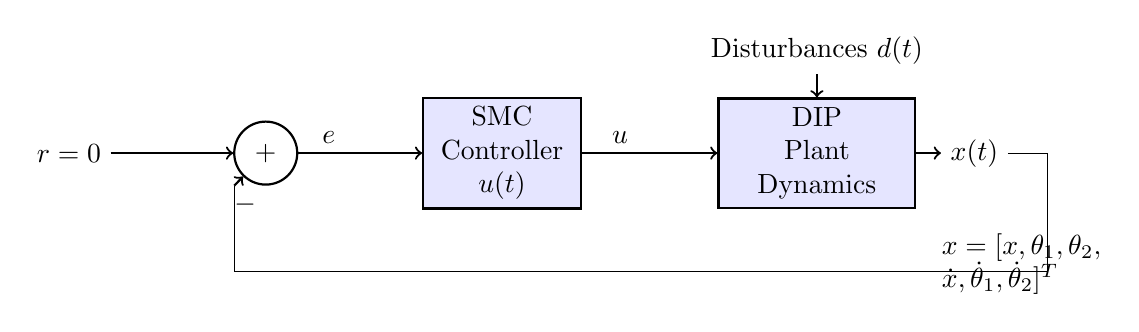
\begin{tikzpicture}[
    block/.style={rectangle, draw, thick, fill=blue!10, minimum height=1cm, minimum width=2cm, align=center},
    sum/.style={circle, draw, thick, minimum size=0.8cm},
    arrow/.style={->, thick},
    node distance=2.5cm
]
    % Reference input
    \node (ref) {$\vect{r} = \vect{0}$};

    % Summing junction
    \node[sum, right of=ref] (sum) {$+$};
    \draw[arrow] (ref) -- (sum);

    % Error signal
    \coordinate[right of=sum, node distance=0.8cm] (err);
    \node[above] at (err) {$\vect{e}$};

    % SMC Controller
    \node[block, right of=sum, node distance=3cm] (controller) {SMC\\Controller\\$u(t)$};
    \draw[arrow] (sum) -- (controller);

    % Control signal
    \coordinate[right of=controller, node distance=1.5cm] (ctrl);
    \node[above] at (ctrl) {$u$};

    % DIP Plant
    \node[block, right of=controller, node distance=4cm, minimum width=2.5cm] (plant) {DIP\\Plant\\Dynamics};
    \draw[arrow] (controller) -- (plant);

    % Output
    \coordinate[right of=plant, node distance=2cm] (output);
    \node[right of=plant, node distance=2cm] (y) {$\vect{x}(t)$};
    \draw[arrow] (plant) -- (y);

    % Feedback path
    \coordinate[below of=plant, node distance=1.5cm] (feedback);
    \draw (y.east) -- ++(0.5, 0) |- (feedback) -| ([xshift=-0.4cm]sum.south);
    \draw[arrow] ([xshift=-0.4cm]sum.south) -- (sum);

    % State labels on feedback
    \node[right, align=left] at ([xshift=0.2cm, yshift=-0.7cm]plant.south east)
        {$\vect{x} = [x, \theta_1, \theta_2,$\\$\dot{x}, \dot{\theta}_1, \dot{\theta}_2]^T$};

    % Disturbances
    \node[above of=plant, node distance=1.3cm] (dist) {Disturbances $d(t)$};
    \draw[arrow] (dist) -- (plant);

    % Negative feedback indicator
    \node[below left] at (sum.south) {$-$};

\end{tikzpicture}
